%----------------------------------------------------------------------------------------
%	PACKAGES AND THEMES
%----------------------------------------------------------------------------------------
\documentclass[aspectratio=169,xcolor=dvipsnames]{beamer}
\usepackage[english,russian]{babel}
\usetheme{Simple}

\usepackage{hyperref}
\usepackage{graphicx} % Allows including images
\usepackage{booktabs} % Allows the use of \toprule, \midrule and \bottomrule in tables

%----------------------------------------------------------------------------------------
%	TITLE PAGE
%----------------------------------------------------------------------------------------

% The title
\title{Улучшение качества видеопотока с помощью нейронных сетей на графических процессорах}
\subtitle{Курсовая работа}

\author[Pin-Yen] {Бинцаровский Леонид Петрович}
\institute[NTU] % Your institution may be shorthand to save space
{
    % Your institution for the title page
    Белорусский государственный университет\\
    ФПМИ, ДМА, 4 курс\\
    руководитель: старший преподаватель Пирштук Д. И.
    \vskip 3pt
}
\date{Минск, 2024} % Date, can be changed to a custom date


%----------------------------------------------------------------------------------------
%	PRESENTATION SLIDES
%----------------------------------------------------------------------------------------

\begin{document}

\begin{frame}
    % Print the title page as the first slide
    \titlepage
\end{frame}

% \begin{frame}{Overview}
%     % Throughout your presentation, if you choose to use \section{} and \subsection{} commands, these will automatically be printed on this slide as an overview of your presentation
%     \tableofcontents
% \end{frame}

%------------------------------------------------
\section{First Section}
%------------------------------------------------

\begin{frame}{Виды улучшения качества видеопотока}
    \begin{columns}[c] % The "c" option specifies centered vertical alignment while the "t" option is used for top vertical alignment

        \column{.45\textwidth} % Left column and width
        \begin{itemize}
            \item Super-resolution (увеличение разрешения)
            \item Стилизация в определенном стиле
            \item Denoising (удаление шума)
            \item Улучшение цветопередачи
            \item Автоматическое центрирование объекта
        \end{itemize}

        \column{.5\textwidth} % Right column and width
        \begin{figure}[h]
            \center{\includegraphics[width=\linewidth]{images/processed.png}}
            \label{ris:Processed}
        \end{figure}
        
    \end{columns}
\end{frame}

%------------------------------------------------

\begin{frame}{Описание модели whitebox\_cartoon\_gan}
    \begin{columns}[c] % The "c" option specifies centered vertical alignment while the "t" option is used for top vertical alignment

        \column{.45\textwidth} % Left column and width
        \begin{figure}[h]
            \center{\includegraphics[width=0.9\linewidth]{images/model.png}}
            \label{ris:ORTModelData}
        \end{figure}

        \column{.5\textwidth} % Right column and width
        \begin{enumerate}
            \item GAN (Генеративно-состязательная сеть);
            \item Генератор представляет собой сеть типа Link-net (U-Net) и делит входное изображение на три представления:
                \begin{enumerate} 
                \item Представление поверхности
                \item Представление структуры
                \item Представление текстуры
                \end{enumerate}
            \item Дискриминатор обеспечивает соответствие сгенерированных изображений требуемому стилю мультфильма, оценивая их подлинность. Применяется только в обучении модели.
        \end{enumerate}

    \end{columns}
\end{frame}

%------------------------------------------------

\begin{frame}{Постановка задачи}
    Для улучшения качества видеопотока с помощью нейронных сетей на графических процессорах будут использоваться:

    \begin{block}{Фреймворк}
        MediaPipe
    \end{block}

    \begin{block}{Модели}
        whitebox\_cartoon\_gan\_360x640.tflite и whitebox\_cartoon\_gan\_640x360.tflite
    \end{block}

    \begin{block}{Языки программирования, среда разработки и операционные системы}
        С++ и Swift, XCode и macOS, Linux, iOS
    \end{block}
\end{frame}


%------------------------------------------------

\begin{frame}{Основные элементы конвейера}
    \begin{columns}[c] % The "c" option specifies centered vertical alignment while the "t" option is used for top vertical alignment

        \column{.45\textwidth} % Left column and width
        \begin{figure}[h]
            \center{\includegraphics[width=0.9\linewidth]{images/graph.png}}
            \label{ris:ORTModelData}
        \end{figure}

        \column{.5\textwidth} % Right column and width
        \begin{enumerate}
            \item FlowLimiterCalculator
            \item ImageToTensorCalculator
            \item InferenceCalculator
            \item TensorToImageCalculator
            \item FromImageCalculator
        \end{enumerate}

    \end{columns}
\end{frame}

%------------------------------------------------

\begin{frame}{Параметры графов для платформ macOS и Linux, iOS}
    \begin{columns}[c] % The "c" option specifies centered vertical alignment while the "t" option is used for top vertical alignment

        \column{.5\textwidth} % Left column and width
        macOS:
        \begin{enumerate}
            \item Модель whitebox\_cartoon\_gan\_360x640.tflite
            \item Делегат XNNPack
            \item Входной/выходной буфер конвейера на CPU
        \end{enumerate}

        \column{.5\textwidth} % Right column and width
        Linux, iOS:
        \begin{enumerate}
            \item Модель whitebox\_cartoon\_gan\_640x360.tflite
            \item Делегат GPU
            \item Входной/выходной буфер конвейера на GPU
        \end{enumerate}
    \end{columns}
\end{frame}

%------------------------------------------------

\begin{frame}{Запуск и тест приложений на платформах macOS, Linux и iOS}
    \begin{columns}[] % The "c" option specifies centered vertical alignment while the "t" option is used for top vertical alignment

        \column{.7\textwidth} % Left column and width
        \begin{figure}[h]
            \center{\includegraphics[width=1\linewidth]{images/macOS.png}}
            \label{ris:ORTModelData}
        \end{figure}

        \column{.3\textwidth} % Right column and width
        \begin{figure}[h]
            \center{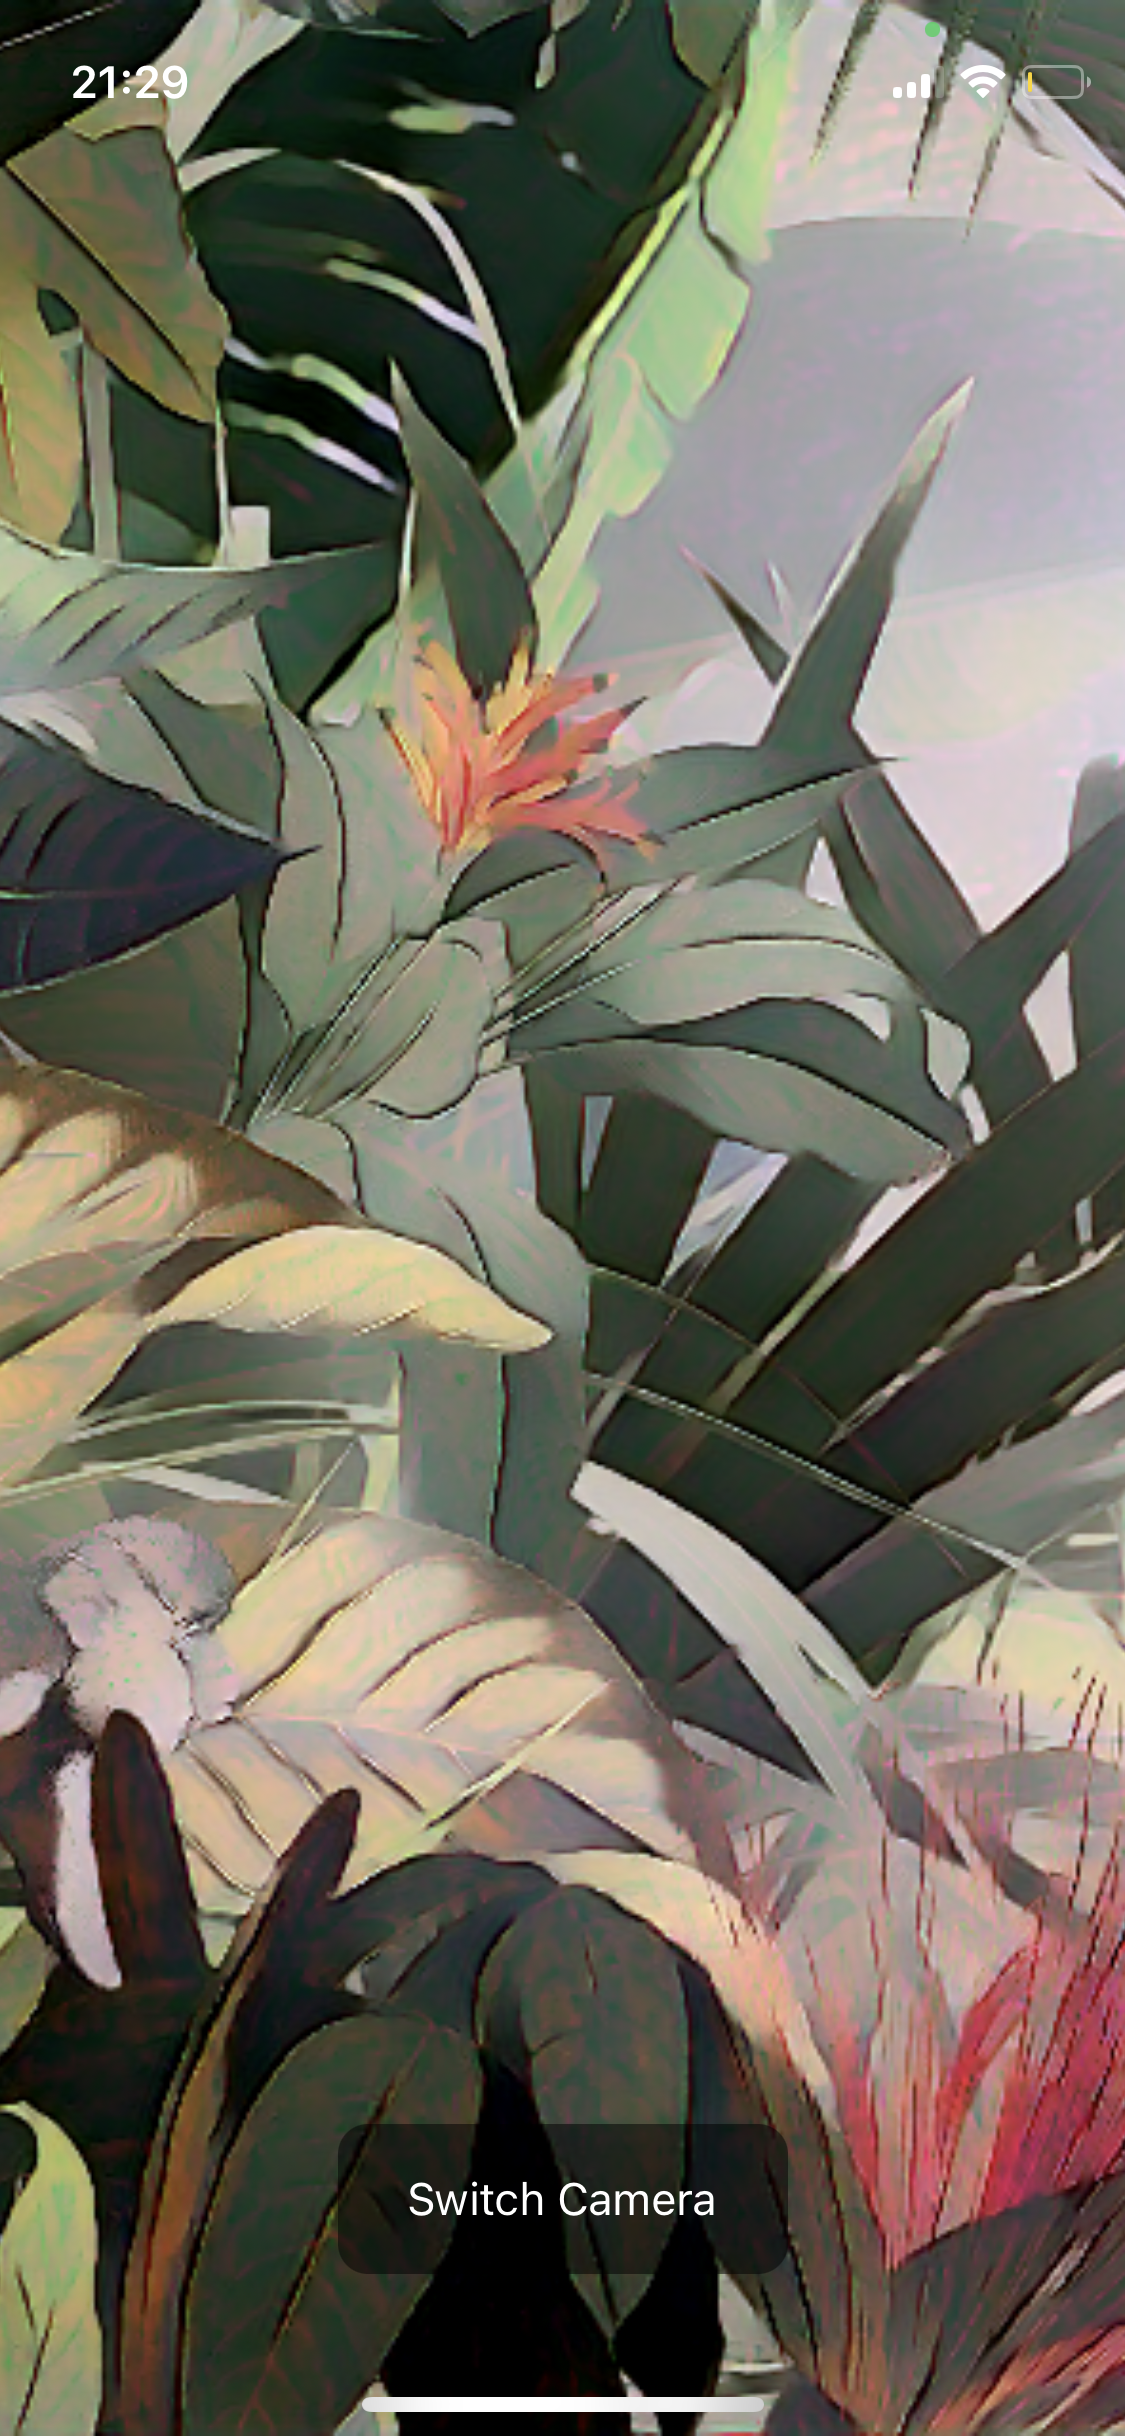
\includegraphics[width=0.65\linewidth]{images/iOS.png}}
            \label{ris:ORTModelData}
        \end{figure}
    \end{columns}
\end{frame}

%------------------------------------------------

\begin{frame}{Выводы}
    \begin{itemize}
        \item Была рассмотрена задача улучшения видеопотока с помощью фреймворка MediaPipe, а также ее применение на прикладном уровне;
        \item Выполнен обзор основных элементов конвейера фреймворка MediaPipe;
        \item Разработана общая архитектура конвейера;
        \item Реализованы конвейеры для платформ macOS, Linux и iOS;
        \item Разработаны приложения для тестирования конвейеров на macOS, Linux и iOS на языках программирования C++ и Swift;
        \item Успешно протестированы результаты работы.
    \end{itemize}
\end{frame}

%----------------------------------------------------------------------------------------

\end{document}